% Note to reader: lines beginning with the '%' character are
% 'comments' to you, the human reader of this code, and are 
% ignored by the LaTeX compiler.

%%%%%%%%%%%%%%%%%%%%%%%%%%%%%%%%%%%%%%%%%%%%%%%%%%%%%%%%%%%%%%%%%%
% = Sample template for MIT Junior Lab Student Written Summaries =
% Available from 
%    http://web.mit.edu/8.13/www/Samplepaper/sample-paper.tex
%
% Last Updated July 23, 2014
%
% Adapted from the American Physical Societies REVTeK-4.1 Pages
%    at http://publish.aps.org
%
% ADVICE TO STUDENTS: Each time you write a paper, start with this
%    template and save under a new filename.  If convenient, don't
%    erase unneeded lines, just comment them out using the 
%    '%' character at the start of the line.  Often, they
%    will be useful containers for information.
%
% Using pdflatex, images must be either PNG, GIF, JPEG or PDF.
%    Turn EPS (encapsulated postscript) images to PDF using the
%    epstopdf utility on UNIX systems.
%%%%%%%%%%%%%%%%%%%%%%%%%%%%%%%%%%%%%%%%%%%%%%%%%%%%%%%%%%%%%%%%%%

%%%%%%%%%%%%%%%%%%%%%%%%%%%%%%%%%%%%%%%%%%%%%%%%%%%%%%%%%%%%%%%%%%
% = TO COMPILE THIS DOCUMENT =
%
% From the command line, it would go like this --- assuming you are
%    in the directory where the filename.tex source file and the 
%    filename.bib bibliography file are located, and that you have 
%    permission to create and write files in that directory:
%      > pdflatex filename
%      > bibtex filename
%      > pdflatex filname
%      > pdflatex filename
%    Yes, you run the command several times. The earlier runs 
%    create auxilliary files which keep track of references,
%    citations, equation and section numberring, etc. The later
%    runs combine the information in these auxilliary files with
%    your source document to create the finished product.
%
% If you are using a GUI LaTeX editor like TeXWorks, then there
%    is probably a menu bar button for pdfLaTeX and another for
%    BibTeX. Hit them in the order indicated above. There is 
%    probably also a 'TeXify' button, or something similarly named,
%    which runs all the above commands in one shot.     
%%%%%%%%%%%%%%%%%%%%%%%%%%%%%%%%%%%%%%%%%%%%%%%%%%%%%%%%%%%%%%%%%%


%%%%%%%%%%%%%%%%%%%%%%%%%%%%%%%%%%%%%%%%%%%%%%%%%%%%%%%%%%%%%%%%%%
%  = PREAMBLE =
% The preamble of a LaTeX document is the set of commands that precede
% the \begin{document} line.  It contains a \documentclass line
% to load the REVTeK-4.1 macro definitions and various \usepackage
% lines to load other macro packages.
%
% ADVICE TO STUDENTS: This preamble contains a suggested set of
%     class options to generate a ``Junior Lab'' look and feel that
%     facilitate quick review and feedback from one's peers, TAs,
%     and section instructors.  Don't make substantial changes 
%     to the style without first consulting your section 
%     instructor.
%%%%%%%%%%%%%%%%%%%%%%%%%%%%%%%%%%%%%%%%%%%%%%%%%%%%%%%%%%%%%%%%%%

%\documentclass[aps,twocolumn,secnumarabic,balancelastpage,amsmath,amssymb,nofootinbib, floatfix]{revtex4}
\documentclass[aps,twocolumn,secnumarabic,balancelastpage,amsmath,amssymb,nofootinbib,floatfix]{revtex4-1}

%%%%%%%%%%%%%%%%%%%%%%%%%%%%%%%%%%%%%%%%%%%%%%%%%%%%%%%%%%%%%%%%%%%
% N.B.:  Different computers have different packages installed.  
%        To compile this template in the current Athena 
%        environment, REVTeX 4.1 must be used.  To use the older
%        REVTeX 4, switch which documentclass line above is 
%        commented out above. There are ``bad'' distributions of
%        LaTeX for Windows available on the internet which may 
%        cause users to struggle unjustifiably with REVTeX 4.1.
%
%        If you are unable to compile the template at all, you
%        may need to update your LaTeX packages. (Alternatively, if 
%        your LaTeX distribution includes only the older RevTEX 4,
%        then try changing the documentclass line above. In particular,
%        this approach solves a common compilation problem for users of
%        the TeXWorks editor on Windows, which presents erroneously as a
%        error in the bibliography file.) Don't hesitate to speak 
%        with your section instructor or a TA if you're having 
%        issues getting this template to compile.
%%%%%%%%%%%%%%%%%%%%%%%%%%%%%%%%%%%%%%%%%%%%%%%%%%%%%%%%%%%%%%%%%%%

%%%%%%%%%%%%%%%%%%%%%%%%%%%%%%%%%%%%%%%%%%%%%%%%%%%%%%%%%%%%%%%%%%%
% = Explanation of documentclass options =
%
% aps, prl stand for American Physical Society and Physical 
%     Review Letters respectively.
% twocolumn permits two columns, of course.
% nobalancelastpage doesn't attempt to equalize the lengths of 
%     the two columns on the last page  as might be desired in a 
%     journal where articles follow one another closely.
% amsmath and amssymb are necessary for the subequations 
%     environment among others. These functionalities can
%     also be added use the usepackage function described below,
%     but REVTeX conveniently includes them as documentclass
%     options.
% secnumarabic identifies sections by number to aid electronic 
%     review and commentary.
% nofootinbib forces footnotes to occur on the page where they are
%      first referenced and not in the bibliography.
% floatfix attempts to help LaTeX decide where to place ``floats'',
%      like figures and plots, when it gets stuck and can't decide
%      by it's normal algorithm.
% REVTeX 4.1 is a set of macro packages designed to be used with 
%      LaTeX 2e. REVTeX is well-suited for preparing manuscripts 
%      for submission to APS journals.
%
% = Other documentclasses =
%
% The 'revtex4' and 'revtex4-1' documentclasses are somewhat 
%    specialized for making documents in the style of the APS
%    journals. For a more standard or generic looking LaTeX paper,
%    you could try any of the built-in documentclasses, in 
%    particular 'article' or 'report'. Someday, you may try to use 
%    the 'mitthesis'  documentclass available for download from the 
%    MIT Libraries. The vast majority of source code written for 
%    one documentclass should work just fine in any other, but 
%    occasional quirks arise. For example, some documentclasses 
%    disagree on whether the abstract declaration should come 
%    before or after the \begin{document} declaration.
% 
%%%%%%%%%%%%%%%%%%%%%%%%%%%%%%%%%%%%%%%%%%%%%%%%%%%%%%%%%%%%%%%%%%%

%% Now, include some packages which provide new commands that 
%% extend LaTeX's capabilities. Note that the nearly-essential
%% AMS math packages were added already as documentclass options
%% for REVTeX, but could have been added here using 
%% \usepackage{amsmath}, etc. The pacakges below are commonly 
%% useful, but there are many, many more available to solve a 
%% multitude of typesetting quandries (google your problem), 
%% and you  probably have the necesary packages installed on your
%% system already. Among the examples listed below, this sample
%% document only actually makes use of the 'graphicx', 'bm', 
%% and 'hyperref' pacakges, so the others are commented out for
%% tidyness.


\usepackage{graphicx}      % tools for importing graphics
%\usepackage{lgrind}        % convert program code listings to a form 
                            % includable in a LaTeX document
%\usepackage{xcolor}        % produces boxes or entire pages with 
                            % colored backgrounds
%\usepackage{longtable}     % helps with long table options
%\usepackage{epsf}          % old package handles encapsulated postscript issues
\usepackage{bm}            % special bold-math package. usge: \bm{mathsymbol}
%\usepackage{asymptote}     % For typesetting of mathematical illustrations
%\usepackage{thumbpdf}
\usepackage[colorlinks=true]{hyperref}  % this package should be added after 
                                        % all others.
                                        % usage: \url{http://web.mit.edu/8.13}


%%%%%%%%%%%%%%%%%%%%%%%%%%%%%%%%%%%%%%%%%%%%%%%%%%%%%%%%%%%%%%%%%%%
% And now, begin the document...
%%%%%%%%%%%%%%%%%%%%%%%%%%%%%%%%%%%%%%%%%%%%%%%%%%%%%%%%%%%%%%%%%%%

\begin{document}
\title{Polarization Topology and Optical Bound States in the Continuum}
\author{Francisco Leal Machado}
\email{fmachado@mit.edu}
%\homepage{http://web.mit.edu/8.13/} %If you don't have one, just comment out this line.
\date{\today}
\affiliation{MIT Department of Physics}


\begin{abstract}
This paper analyzes how optical modes in photonic crystal slabs can decouple from the environment continuum of radiation through topological protected vortices in the polarization of outgoing radiation. We review previous work done in this area \cite{Zhen2014, hSU2013} developing the idea of a polarization field on the Brillouin zone and analyze how the topology, in particular the winding, of this field implies the existence of a bound state in the continuum (BIC).  We analyze photonic crystal slabs periodic in one direction and extended the other in order to demonstrate the existence of these theorized modes and their robustness to perturbations which do not break the symmetries of the system. Departing from previous literature, we also analyze the effect of symmetry breaking in the polarization field and the resonant modes of the system and show the existence of topological half-charge modes in when $\sigma_z$ symmetry is broken.
\end{abstract}

\maketitle

\section{Introduction}

The field of photonic crystals (PhCs), periodic structures at the lengthscale of light, has undergone a great development in recent years, with amazing results in the way we understand and engineer the flow of light. This body of work has resulted in many applications ranging from new devices such as novel narrow-band filters to control of the direction of light at the wavelength scale 
\cite{D.Joannopoulos2008}  as well as the realization of novel phenomena like the chiral propagation of light \cite{Wang2009} and the realization of systems with Weyl points \cite{Lu2013, Lu2015}.

A topic of particular interest to engineering applications is the realization and control of bound states in the continuum (BIC). In real life applications, often one uses light whose momentum and energy enable it to travel in free-space. Unfortunately, that means that resonant modes in PhC slabs are capable to couple to free space radiation modes and decay over time, preventing their propagation over very large distances. Fortunately, BICs correspond to modes completely uncoupled from the outside continuum of radiation, enabling them to be long lived. As a result, begin able to predict and engineer these modes opens the doors for new application of PhC technology.

BICs were initially proposed by von Neumann and Wigner \cite{von1929unusual} in the context of Quantum Mechanics, through the description of very complex potentials. As a result from this complexity, these BIC were not robust under perturbations of the potential making them experimentally elusive. More recent work had analyzed BIC that arise from a symmetry mismatch between the bound state and the continuum modes, which prevent the BIC to leak couple to the continuum degrees of freedom \cite{Evans2006, Rivera2015}. In this paper we analyze a new approach, proposed and observed in Zhen's paper, and then explained in the context of topology in a following work  \cite{Zhen2014, hSU2013}. We go further from the literature and study the effect of breaking the symmetries which protect the topological properties and uncover the existence of topological half-charge points.


\section{Theoretical Background}
\label{sec:sym}
% Master equation

% Introduction to Bloch Theorem


Although Maxwell's equations remain the same since their proposal in the 1860', the approach used to solve them has suffered a tremendous evolution in the last decades. Making use of knowledge from group theory, the role of symmetries has been expanded in the study of electromagnetism, allowing scientist to make much more powerfull statements and predictions.

In the case of photonic crystals, the existence of discrete (or continuous) translation symmetries, means that the solutions can be labeled by their momentum within the Brillouin Zone (BZ) of the system. This treatment, analogous to the treatment of the Schr\"{o}dinger equation of electrons in solids, enables us to think of a particular field realization in the PhC as a superposition of modes at different momentum and energy. By solving the equation for each value of momentum of the BZ, the general solution obtained through the superposition of these modes. The electric field $E_{\bm{k}}$ for momentum mode solved through the eigenvalue problem \cite{D.Joannopoulos2008}:
\begin{equation} \label{eq:Maxwell}
  \frac{1}{\epsilon} (\nabla + i\bm{k})\times (\nabla + i\bm{k})\times \bm{u}_{\bm{k}} = \omega^2  \bm{u}_{\bm{k}}
\end{equation}

\noindent where $\bm{k}$ is the momentum of the mode, $\bm{u}_{\bm{k}}$ is a periodic function in the unit cell of our crystal related to the electric field by $\bm{E}_{\bm{k}} = e^{i\bm{k}\cdot\bm{x}} \bm{u}_{\bm{k}}$, $\bm{x}$ is the position and $\epsilon$ is the electric permittivity of the material. Throughout this paper we will be working in units where the speed of light, the vacuum electric permittivity and the magnetic permeability are all 1,  $c=\epsilon_0=\mu_0=1$. We also only consider materials whose magnetic permeability matches the vacuum, $\mu = \mu_0$ a good approximation to most materials.

One interesting realization of PhC systems is the PhC slab which corresponds to a thin cross-section of a two dimensional crystal, as depicted in Fig.(\ref{fig:schematic}). Although in the direction of the surface, there is discrete translation symmetry, no translation symmetry is found in the out of plane direction ($\hat{z}$), meaning that there is no meaningful momentum in the out of plane direction. Moreover the existence of free space around the slab leads to the coupling of the modes within the slab to free space radiation with matching energy and in-plane momentum. As a result, instead of modes that are able to live indefinitely in the slab (considering the lossless regime), modes decay by ``leaking'' out into free space radiation, and instead of pure modes of the system we observe discrete resonances. These resonances, although not infinitely lived modes, are modes which become trapped in the PhC and slowly decay. To quantify the lifetime of a resonance, the quality factor $Q$ is used, defined as:
\begin{equation}
  Q = -\frac{\text{Re}(\omega)}{2\text{Im}(\omega)}
\end{equation}

\noindent where Re$(\omega)$ (Im$(\omega)$) is the real (imaginary) part of $\omega$, the frequency of the mode, which dictates the evolution of the mode as $e^{-i\omega t}$. $Q$ can be interpreted as the number of oscillations the mode undergoes before decaying.

For a particular mode, with in-plane momentum $\bm{k}$ and frequency $\omega$, by conservation of momentum and energy, it can only couple to outgoing radiation which travels in the direction of $\bm{k}_{rad} = (k_x, k_y, \pm\sqrt{\omega^2 - \bm{k}^2})$. However the polarization of the radiation can take any value and in general will be elliptical. In order to compute the radiation polarization we note that the electromagnetic field, in the far field, will be given by:
\begin{align}
  \bm{E}_{rad} \propto \hat{E} e^{i\bm{k}_{rad}\cdot \bm{r}}& = \hat{E} e^{i(\bm{k}\cdot \bm{\rho}} e^{i \sqrt{\omega^2 - \bm{k}^2} z}\\
& \Rightarrow \hat{E} \propto \bm{E}_{rad} e^{-i\bm{k}\cdot \bm{\rho}} = \bm{u}_k 
\end{align} 

\noindent where $\hat{E}$ is the polarization of the electric field, $\rho$ is the in-plane position, $z$ is the out of plane position. Since $\hat{E}$ is a constant, while $\bm{u}_k$ varies within the unit cell, due to near-field effects, we integrate the $\bm{u}_{\bm{k}}$ for a fixed $z$ over the unit cell, at the far-field position. This provides a more robust method for computing the polarization:
\begin{equation} \label{eq:coup}
  \bm{c}_k = \int_{z=cte} \bm{u}_{\bm{k}} = \langle \bm{u}_{\bm{k}}\rangle
\end{equation}

Another way of thinking about why the integration over the unit cell is necessary is to think that we want to understand the coupling of our system to the far-field radiation, so we should compute the inner product between the two, leading to an integration over the BZ for a fixed $z$. Although coupling to higher modes of outside radiation is possible we restrict ourselves to be above the first light cone and below the second one, where only the coupling arising in \ref{eq:coup} can occur. 

Of interest is the in-plane projection of the polarization vector, since the $z$ component is fully determined by the orthogonality of the propagation and the polarization vector. More importantly, if the in-plane polarization is $0$, there is no energy flux away from the slab, as the radiation is parallel to the surface.

For a general Phc slab, the polarization of the radiative field can take any value. However if we impose extra symmetries in our system we will also impose certain restrictions on the form of the electromagnetic modes of the system, which restrict the polarization of our system.

The existence of a translation symmetry already imposed a constraint in the solution for our modes into Bloch modes. Now we analyze the effect of $C_2^z T$, time reversal and rotation around the $z$ axis by $\pi$, and $\sigma_z$, reflection around the $z=0$ plane, on the electromagnetic modes. Since the geometry of our system is dictated by the value of the electric permitivitty in space, $C_2^zT$ symmetry corresponds to having:
\begin{equation}
\epsilon(x,y,z) = \epsilon^*(-x,-y,z)
\end{equation}

\noindent where $\epsilon^*$ is the complex conjugate of $\epsilon$. $\sigma_z$ symmetry corresponds to:
\begin{equation}
  \epsilon(x,y,z) = \epsilon(x,y,-z)
\end{equation}

We now show how these symmetries impose constraints on $\bm{u}_{\bm{k}}$, associated with the transformations of the field. In particular $C_2^zT$ implies that if $\bm{u}_{\bm{k}}(\bm{r})$ is a solution, $C_2^zu^*(C_2^z \bm{r})$ is also a solution. To see this we write:
\begin{align}
  &\frac{1}{\epsilon(\bm{r})} (\nabla + i\bm{k})\times (\nabla + i\bm{k})\times C_2^z\bm{u}^*(C_2^z \bm{r})=\\
  & C_2^z\frac{1}{\epsilon(\bm{r})} ((-\hat{x}\partial_x - \hat{y}\partial_y + \hat{z}\partial_z) - i\bm{k})\times\notag\\
  &\times ((-\hat{x}\partial_x - \hat{y}\partial_y + \hat{z}\partial_z) - i\bm{k})\times \bm{u}^*(C_2^z \bm{r})=\notag\\
  & C_2^z\frac{1}{\epsilon^*(C_2^z\bm{r})} (\nabla_{C_2^z\bm{r}} - i\bm{k})\times (\nabla_{C_2^z\bm{r}} - i\bm{k})\times \bm{u}^*(C_2^z \bm{r})=\notag\\
  & C_2^z\left[\frac{1}{\epsilon(C_2^z\bm{r})} (\nabla_{C_2^z\bm{r}} + i\bm{k})\times (\nabla_{C_2^z\bm{r}} + i\bm{k})\times \bm{u}(C_2^z \bm{r})\right]^*\notag\\
  & \quad \quad= (\omega^2)^* C_2^z \bm{u}^*(C_2^z \bm{r})
\end{align}

For our statement to be true $\omega$ must be purely real for $\omega^2 = (\omega^2)^*$. This only occurs when the system is Hermitian, meaning that the system is not open (the slab does not radiate) and we have a bound mode. However if we consider modes nearby our BIC, we can approximate $\omega^2 \approx (\omega^2)^*$.

Since the irreducible representations of $C_2^z$ have one dimension,$ \bm{u}_{\bm{k}}$ and $C_2^z \bm{u}^*(C_2^z \bm{r})$  must correspond to the same solution up to a phase, $e^{i\phi}$, which we can choose to be $-1$ due to the arbitrariness of phase. This guarantees that the zero Fourier term of $\bm{u}_{\bm{k}}$ real in the $x$ and $y$ direction and purely imaginary in the $z$ direction:
\begin{equation}
  \bm{c}_{\bm{k}} = \int d\bm{r} \bm{u}_{\bm{k}}(\bm{r}) = \int_{x>0} d\bm{r} (\bm{u}_{\bm{k}}(\bm{r}) - C_2^z \bm{u}_{\bm{k}}^*(\bm{r}))
\end{equation}

Note that had we chosen a different phase value, the same result could be obtained by applying an overall phase shift to the modes. The importance of this procedure is that it imposes a constraint between the real and imaginary part of the of the polarization of the field. Again, although this is strictly not true at points different from the BIC, near them it is true. Far away we will observe that the polarization is not strictly linear, but gains a small ellipticity.

We can show a similar result for $\sigma_z$, by demonstrating that $\sigma_z \bm{u}(\sigma_z \bm{r})$ is a solution if $\bm{u}_{\bm{k}}$, commuting $\sigma_z$ through the cross product and then writing as function of $\bm{u}_{\bm{k}}(\sigma_z \bm{r})$. In this case, the application of the symmetry operation twice brings us to the initial state, which means that the phase must be $\pm 1$. This means that the polarization of the radiation leaking through the top of the PhC matches the polarization of the radiation leaking through the bottom of the slab.

By understanding the coupling to the radiation continuum based on the polarization of the outgoing radiation, the topology of the polarization field provides a new understanding and a new way of considering robust BIC modes in the system. Consider a polarization field which winds, meaning that under a closed loop, the polarization of the radiation turns by an integer number of turns, as depicted in Fig.(\ref{fig:polarization}). Since the polarization has fixed length, and continuously changes within the BZ, if there is a non-zero winding, there must exist a point, where the polarization is not-defined, much like a vortex in water must have a point whose angular velocity is ill-defined (the center) . At these points in $k$-space, the mode becomes a BIC and not just a resonant mode, since there is no radiation which the mode can couple to.

As a result, associated with the winding of the polarization around a contour there is a topological invariant, robust to local perturbations, which corresponds to a topological charge $q$ inside the contour $C$ given by:
\begin{equation}\label{eq:charge}
  q = \frac{1}{2\pi} \oint_{C} d\bm{k} \cdot \nabla_{\bm{k}} \phi(\bm{k}), \quad q\in \mathbb{Z}
\end{equation}

\noindent where $\phi(\bm{k}) = arg[c_x + i c_y]$. At places where the polarization is not strictly linear, the direction of the major axis provides a good measure of the direction of the polarization and enables us to still discuss a winding of the polarization. Eq.(\ref{eq:charge}) can be understood analogously to Gauss's law and point charged particles, meaning that the topological charges will have a point-like position in the BZ, which will correspond to locations of BIC and explains why the system is robust to local perturbations. Eq.(\ref{eq:charge}) also provides a recipe for finding BIC in a PhC slab system. By looking a the global polarization landscape, if the contour integral has a non-zero $q$, then there must be at least one BIC point in the system. Note that $q=0$ does not exclude the possibility of a BIC, as the chosen path may include a point with charge $+1$ and a point with charge $-1$, both corresponding to BICs but whose contour integral will be zero, as the effect of charges add up.


This formalism in terms of the topological properties of the polarization field provides a connection with topics in other fields of Physics, like Quantum Field Theory and Condensed Matter Theory.


% Leaky Modes

% Computing polarization

% Symmetry argument

% Connection to pological Charge



\begin{figure}
\centering
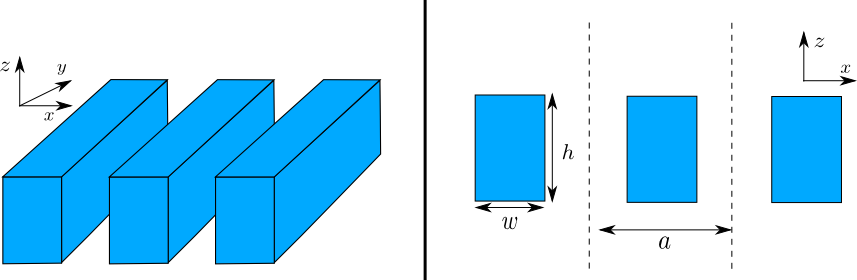
\includegraphics[width=0.5\textwidth]{Figures/schematic.png}
  \caption{{\bf Schematic of the Geometry of Interest.} In this project we restrict ourselves to two dimensional geometries, extended in the $y$ direction, and periodic in the $x$ direction. Throughout this project we change the height $h$ of the slab to investigate the different phenomena. We set $w/a = 0.45$ for all computations.}
  \label{fig:schematic}
\end{figure}



\begin{figure}
  \centering
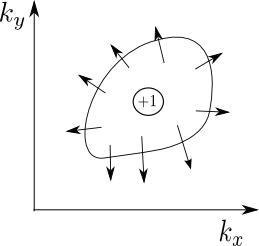
\includegraphics[width=0.3\textwidth]{Figures/polarization.png}
\caption{{\bf Winding of the polarization field.} If the polarization rotates as we move around a closed loop, then inside the loop there must be a topological charge where the polarization is not defined. This will correspond to a BIC.}
\label{fig:polarization}
\end{figure}

\section{Topological Polarization Charge}

% Configuration 3c
In this section we analyze the polarization field for a particular PhC slab geometry and demonstrate the existence of a winding in the polarization associated with BICs in the system. The geometry we will analyze corresponds to a sequence of dielectric square rods finite in the $x$ and $z$ direction and infinite in the $z$ direction, as pictured in Fig.(\ref{fig:schematic}).

The band structure of this structure is pictured in Fig.(\ref{fig:Band}) to guide our choice of bands to analyze. In particular we notice that the lowest band for both transverse magnetic (TM) and transverse electric (TE) is located below the light cone, as expected from the introduction of a higher dielectric material than vacuum in the system, which is cannot couple to a continuum of states, hence won't support BICs.

\begin{figure}
\centering
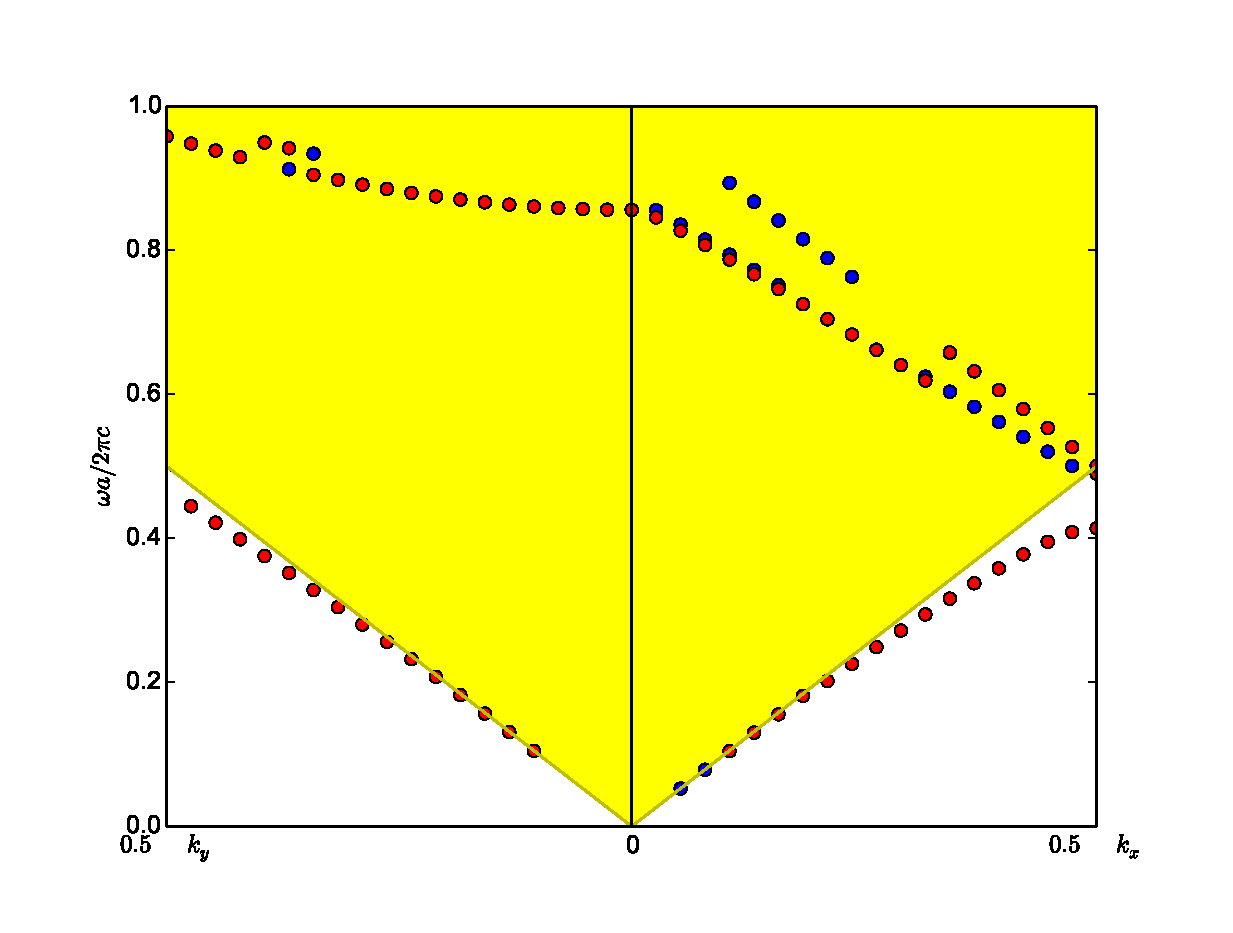
\includegraphics[width=0.5\textwidth]{Figures/BandDiagram.eps}
  \caption{{\bf Band Structure of the PhC slab geometry from Fig.(\ref{fig:schematic}).} In red the TE mode and in blue the TM mode. We are interested in BIC so we must restrict our search for bands higher than the bottom band. This band structure was computed for $h/a = 1.5$.}
  \label{fig:Band}
\end{figure}


We begin by investigating the first TM mode band. Since our system does not only have $TC_2^z$ but also $C_2^z$ symmetry the BZ will be symmetric under $C_2^z$ too. Looking for $h/a = 1.5$, the obtained values of $Q$ for the modes is given in Fig.(\ref{fig:TMModes}). Due to computational constraints, it was impossible to better resolve the divergence in $Q$. However from sharp increase in $Q$ associated with the winding in the polarization we expect a state with $Q\to\infty$ to exist within the contour. In Fig.(\ref{fig:TMModes_change}), we change the height of the slab to $h/a=1.4$ and again compute the $Q$ of the system for the TM modes. There is qualitative change in the position of the BIC, from lying in the $x$ axis to the $y$ axis, but they are still present. In fact performing calculations at intermediate heights, we expect them to continuously move from the position in Fig.(\ref{fig:TMModes}) to the position in Fig.(\ref{fig:TMModes_change}). Due to the topological protection of the polarization, the BIC will be preserved for all perturbations that preserve the symmetries of the system.

\begin{figure}
\begin{minipage}{0.5\textwidth}
  \centering  
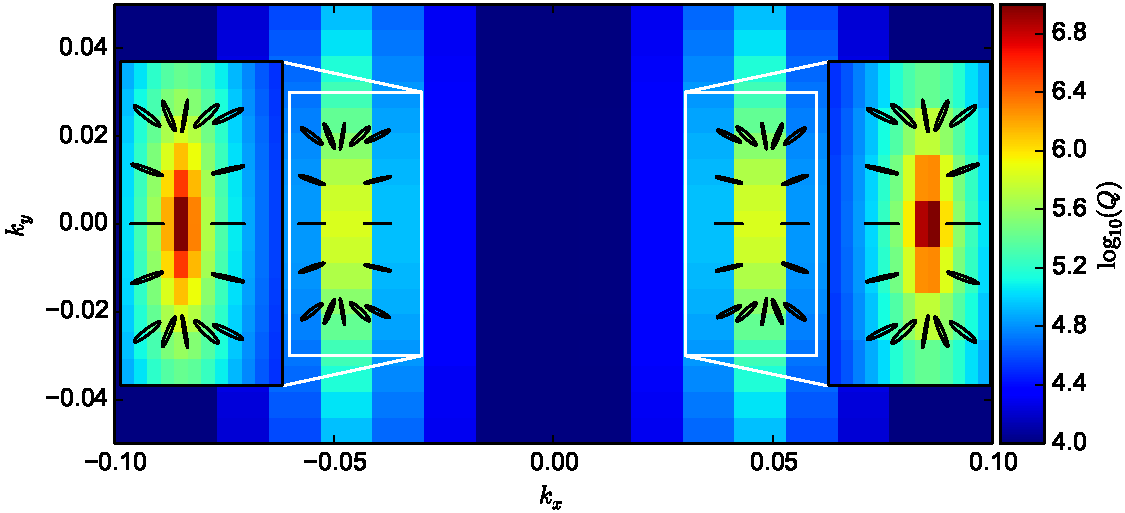
\includegraphics[width=\textwidth]{Figures/h1_5-eps-converted-to-cropped.pdf}
  \caption{{\bf Signs of a divergence in quality factor for $h/a = 1.5$.} Plot of the quality factor for the first TM mode band in the geometry of Fig.(\ref{fig:schematic}). The insets correspond to a higher sampling of the regions of interest. The lines in white correspond to the polarization of the emitted radiation for the corresponding mode. Although the polarization is not strictly linear, it is still possible to see the winding of the polarization around the loops around the point of interest. The peak in $Q$ by many of orders of magnitude matches the location where there is a topological charge, supporting the claims that a BIC is present associated with a non-trivial topology of the polarization field. Further numerical studies are required to confirm that it is in fact a divergence.}
  \label{fig:TMModes}
\end{minipage}
\begin{minipage}{0.5\textwidth}
  \centering  
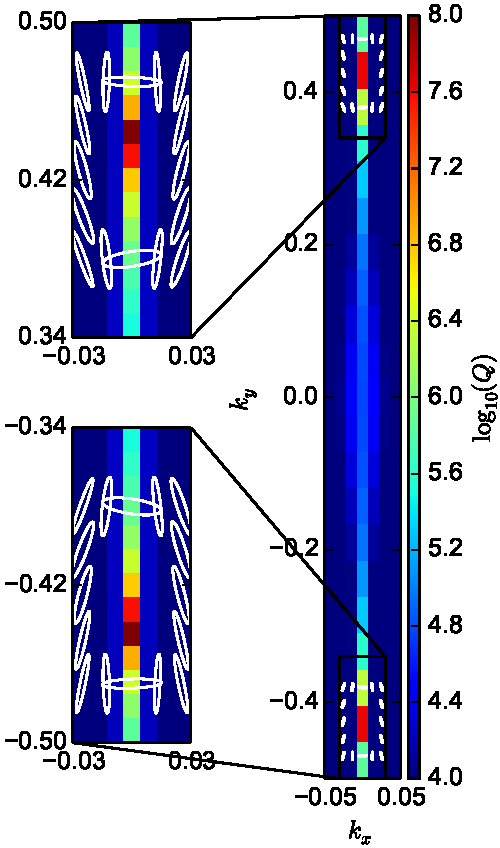
\includegraphics[width=0.5\textwidth]{Figures/h1_4-eps-converted-to-cropped.pdf}
  \caption{{\bf Robustness of BIC with parameter change.} Since the BIC are protected because of the topology of the polarization field, any perturbation that does not break the symmetries of the system.  In this case changing the height of the slabs to $h/a = 1.4$, does not destroy the BIC but moves them into the $y$ axis in $k$-space.}

  \label{fig:TMModes_change}
\end{minipage}
\end{figure}


The same procedure also extends to TE modes. Looking at the first TE band for the slab geometry with $h/a=1.1$ and $h/a=1$. Of interest in this case is how the polarization winds around the side BIC opposite to what was observed in Fig.(\ref{fig:TMModes}), corresponding to a topological charge with opposite sign. After we decrease the height of the slab, the topological charges merge, and the result is a single charge with sign opposite to Fig.(\ref{fig:TMModes}).

Within these two examples we were able to show the robustness of the BIC to perturbations, as well as demonstrate the dynamics of the topological charges, opposite charges can cancel each other.

\begin{figure}
\begin{minipage}{0.5\textwidth}
  \centering  
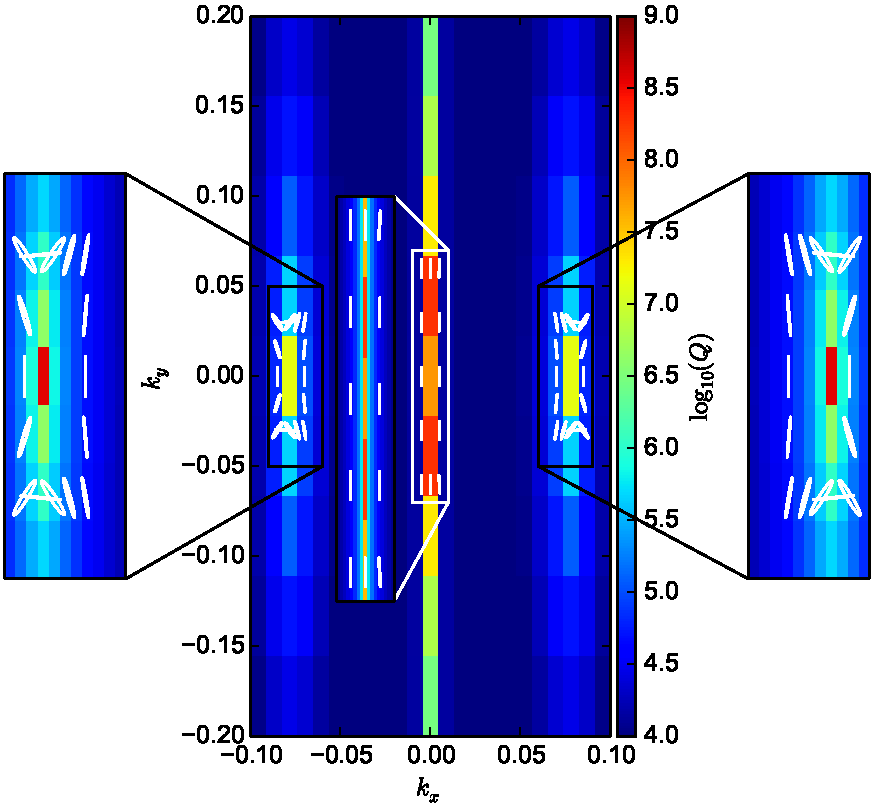
\includegraphics[width=\textwidth]{Figures/h1_1-eps-converted-to-cropped.pdf}
\end{minipage}
\begin{minipage}{0.5\textwidth}
  \centering  
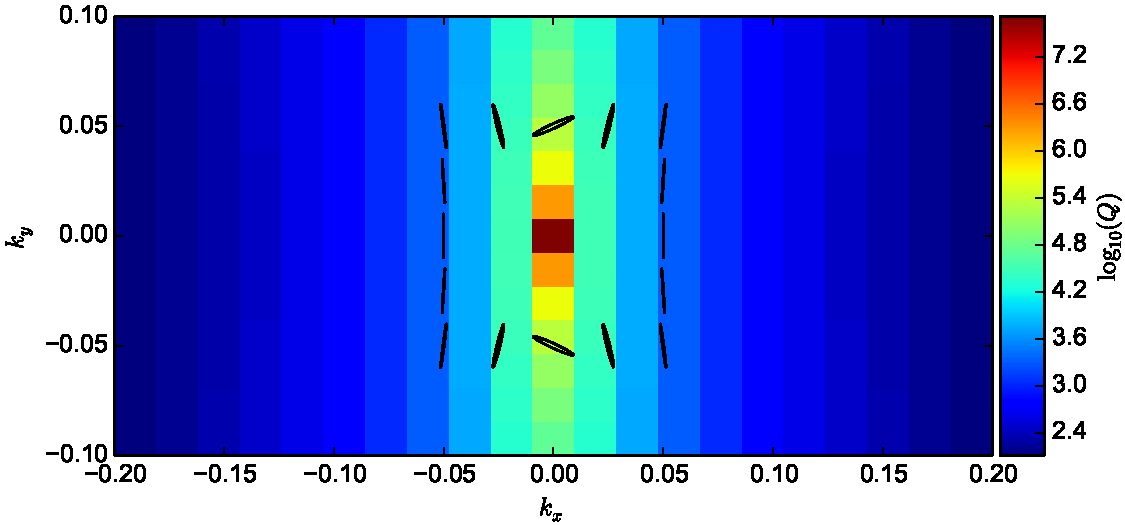
\includegraphics[width=\textwidth]{Figures/h1-eps-converted-to-cropped.pdf}
\end{minipage}
  \caption{{\bf Observation of BIC in TE modes.} Computing the quality factor TE modes of a slab with $h/a = 1.1$ (above) and $h/a=1$ (below) also yields BICs, again protected by the winding of the polarization field. Since the center mode and the side modes have different sign, when we change the height of the system, two topological charges cancel one another and only a single charge remains.}
  \label{fig:TEModes}
\end{figure}

% New Geometry

% Break Symmetry


\section{Breaking $\sigma_z$ Symmetry}

Having shown the existence of BIC arises from the topology of the polarization of the ``leaked'' radiation, we now move our attention into how robust the system is under breaking of the symmetry. In particular we will look at a system where $\sigma_z$ symmetry has been broken. For that we consider a system related to Fig.(\ref{fig:schematic}) where the bottom half of the system has a different electric permittivity from the top half, as pictured in Fig.(\ref{fig:broken_sym}).

\begin{figure}
\centering
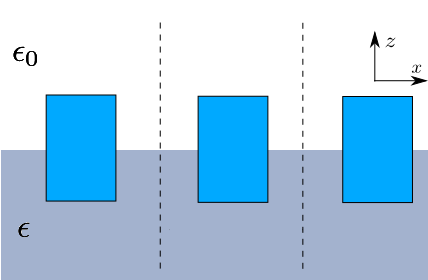
\includegraphics[width=0.35\textwidth]{Figures/broken_symmetry.png}
  \caption{{\bf Breaking the $\sigma_z$ symmetry.} In order to study the effect of the symmetries of the system being broken we analyze the case when the bottom half of the system ($z<0$) is surrounded not by vacuum (whose electric permittivity is $\epsilon_0$) but a material with a different dielectric constant $\epsilon$.}
  \label{fig:broken_sym}
\end{figure}

The result of our calculations are presented in Fig.(\ref{fig:sigma_z}), for a fixed height $h/a = 1.5$, and varying bottom electric permittivity from $1$ (matching the top half) to $1.1$, from left to right. Since the $\sigma_z$ symmetry is broken, we plot the polarization of the top (white lines) and the bottom radiation (black lines).

There are few interesting facts that are worth mentioning. First and foremost we obtain a decoupling between the polarizations between both sides of the slab. This was expected based on our derivation in Sec.(\ref{sec:sym}). What is less expected is how the two polarizations seem to turn in opposite directions. Although, we are not confident of a full explanation of this phenomena, it seems to suggest that as the two sides become more different, each moves into opposite side of the line $c_x=0$ they occupied in the unperturbed system.

The other interesting point is how the polarization become much more elliptical, despite the $C_2^z T$ symmetry still being present. This is most likely due to the fact that we no longer have a $\bm{k}$ where the system is Hermitian and where nearby the polarizations need to be linear.

The most peculiar consequences of this phenomena is the emergence of circularly polarized modes, associated with half-charge points in the BZ. These points are labeled by the red stars, around which we see the circular polarization in white. Demonstrating they correspond to a half-charge phenomena is more complicated due to the width of the elliptical  polarizations, however following the dashed red contour we can see the ellipses performing an half rotation. For a clearer contour we would have to have gone to momentum further away from the initial BIC, which was unfortunately impossible due to computational constraints.

As we increase the perturbation the rotation of the polarizations becomes more clear, hinting again at a distancing of both radiation from the $c_x=0$ line.

\begin{figure}
  \centering  
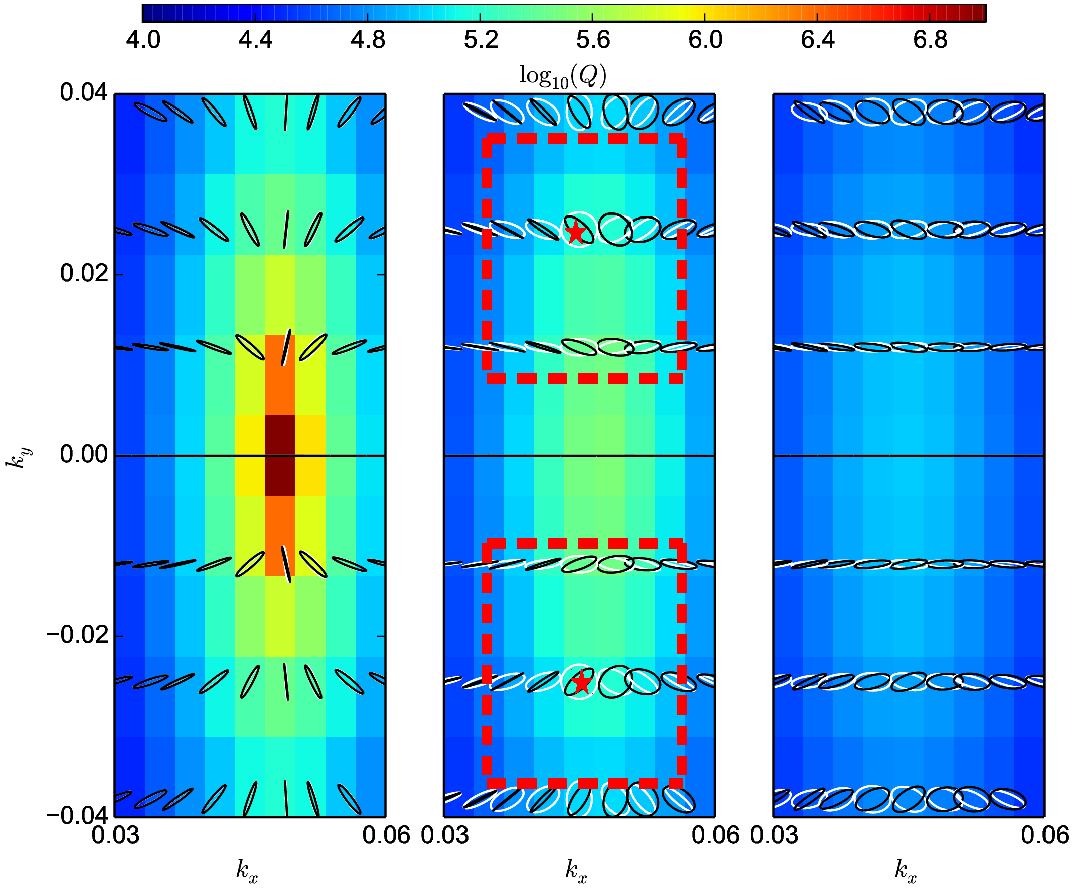
\includegraphics[width=0.5\textwidth]{Figures/Sigma_z_all-cropped.pdf}
  \caption{{\bf Signs of Half-Charge Points in Perturbed Systems.} When the $\sigma_z$ symmetry of the system is broken, in this case by changing the background permittivity of the lower half of the system ($\epsilon = (1,1.05, 1.1)$ from left to right) as depicted in Fig.(\ref{fig:broken_sym}), the polarizations of the radiation leaked through each of the two sides of the slab becomes different. The resulting polarization field, becomes gains a greater ellipticity and rotates. An interesting phenomena that arises are points of half-charge, marked with the red stars. By following the red contours, the polarization rotates only half a turn. Note that there is one is the upper and one in the lower plane of the BZ, and they arise from the separation integer charge BIC point from the unperturbed case (on the left). Note that this is valid, since the polarization can be reversed without destructive interference, if accompanied by a phase shift of the system, which we do not track in this work.}
  \label{fig:sigma_z}
\end{figure}

\section{Conclusion}

In this project we reviewed the work presented in \cite{Zhen2014} and then looked at the case when the $\sigma_z$ symmetry is broken. We developed the concept of the polarization field across the Brillouin zone as the polarization of the electric field of the outgoing radiation associated with the decay of a resonant mode of the photonic crystal slab. Looking at the topology of this field, we discussed the impact of winding of the polarization around a contour, and how they give rise to topologically protected bound states in the continuum (BIC). We showed the existence of the BIC through numerically calculations of a real structure, and showed they were associated with the winding of the polarization field. We then analyzed the impact of breaking the $\sigma_z$ symmetry and we observed the loss of the BIC as well as the topological charge point. However we observe the separation of the topological charge into two half charge points, which move into different half-planes of the Brillouin Zone, associated not with ill-defined polarization but with circular polarization.

The code and data used in this project is available in \url{https://github.com/Lactor/18.369Project}

\section{Acknowledgments}

I would like to thank Prof. Steven G. Johnson for a great class that taught me not only the formalism but also the intuition and beauty behind nanophotonics systems and Maxwell's equations. I would also like to Dr. Bo Zhen for his availability and Hengyun (Harry) Zhou for his enthusiasm and help throughout the project, and pointing the possible existence of the half-charged points in the $\sigma_z$ symmetry broken system.


%%%%%%%%%%%%%%%%%%%%%%%%%%%%%%%%%%%%%%%%%%%%%%%%%%%%%%%%%%%%%%%%%%
\bibliography{paper}


%%%%%%%%%%%%%%%%%%%%%%%%%%%%%%%%%%%%%%%%%%%%%%%%%%%%%%%%%%%%%%%%%%%%%%%%%%%%%
\clearpage
\appendix

\end{document}




























